\subsubsection{Cube ou continuation}
L'opérateur C présente des limites quand à son utilisation, dans le cas d'un graphe structuré à $n$ dimensions, il supprimera une dimension.
%
Or, si nous avons un graphe à 2 dimensions, il supprimera la dimension qui permet d'avoir du parallélisme.
%
Son avantage étant d'optimiser les effets caches à l'intérieur d'une tâche grossière.
%
Pour garder cette avantage, nous avons repris l'algorithme de l'opérateur C et nous avons ajouté un paramètre pour limiter la taille des tâches.
%



Cet opérateur a été créé pour être une réponse efficace à nos problèmes.
%
Dans notre cas, le graphe à ordonnancer à exactement la même structure que le réservoir que nous souhaitons modéliser.
%
La plupart du temps, ce modèle sera un cube 3D.
%
En numérotation naturelle et avec un modèle 3D, une bonne agrégation consiste à agréger toutes les tâches d'un axe qui ont les mêmes coordonnées sur les deux autres axes.
%
Cela correspond à {\em aplatir} notre modèle 3D en un modèle 2D (Fig.~\ref{fig:cube5_algo_C}).
%
Par exemple, un cube de 5 éléments de coté, soit 125 tâches, sera transformé en un carré de 5 éléments de coté, soit 25 tâches.


%   (-_-)   %
\begin{figure}[t!]
  \centering
  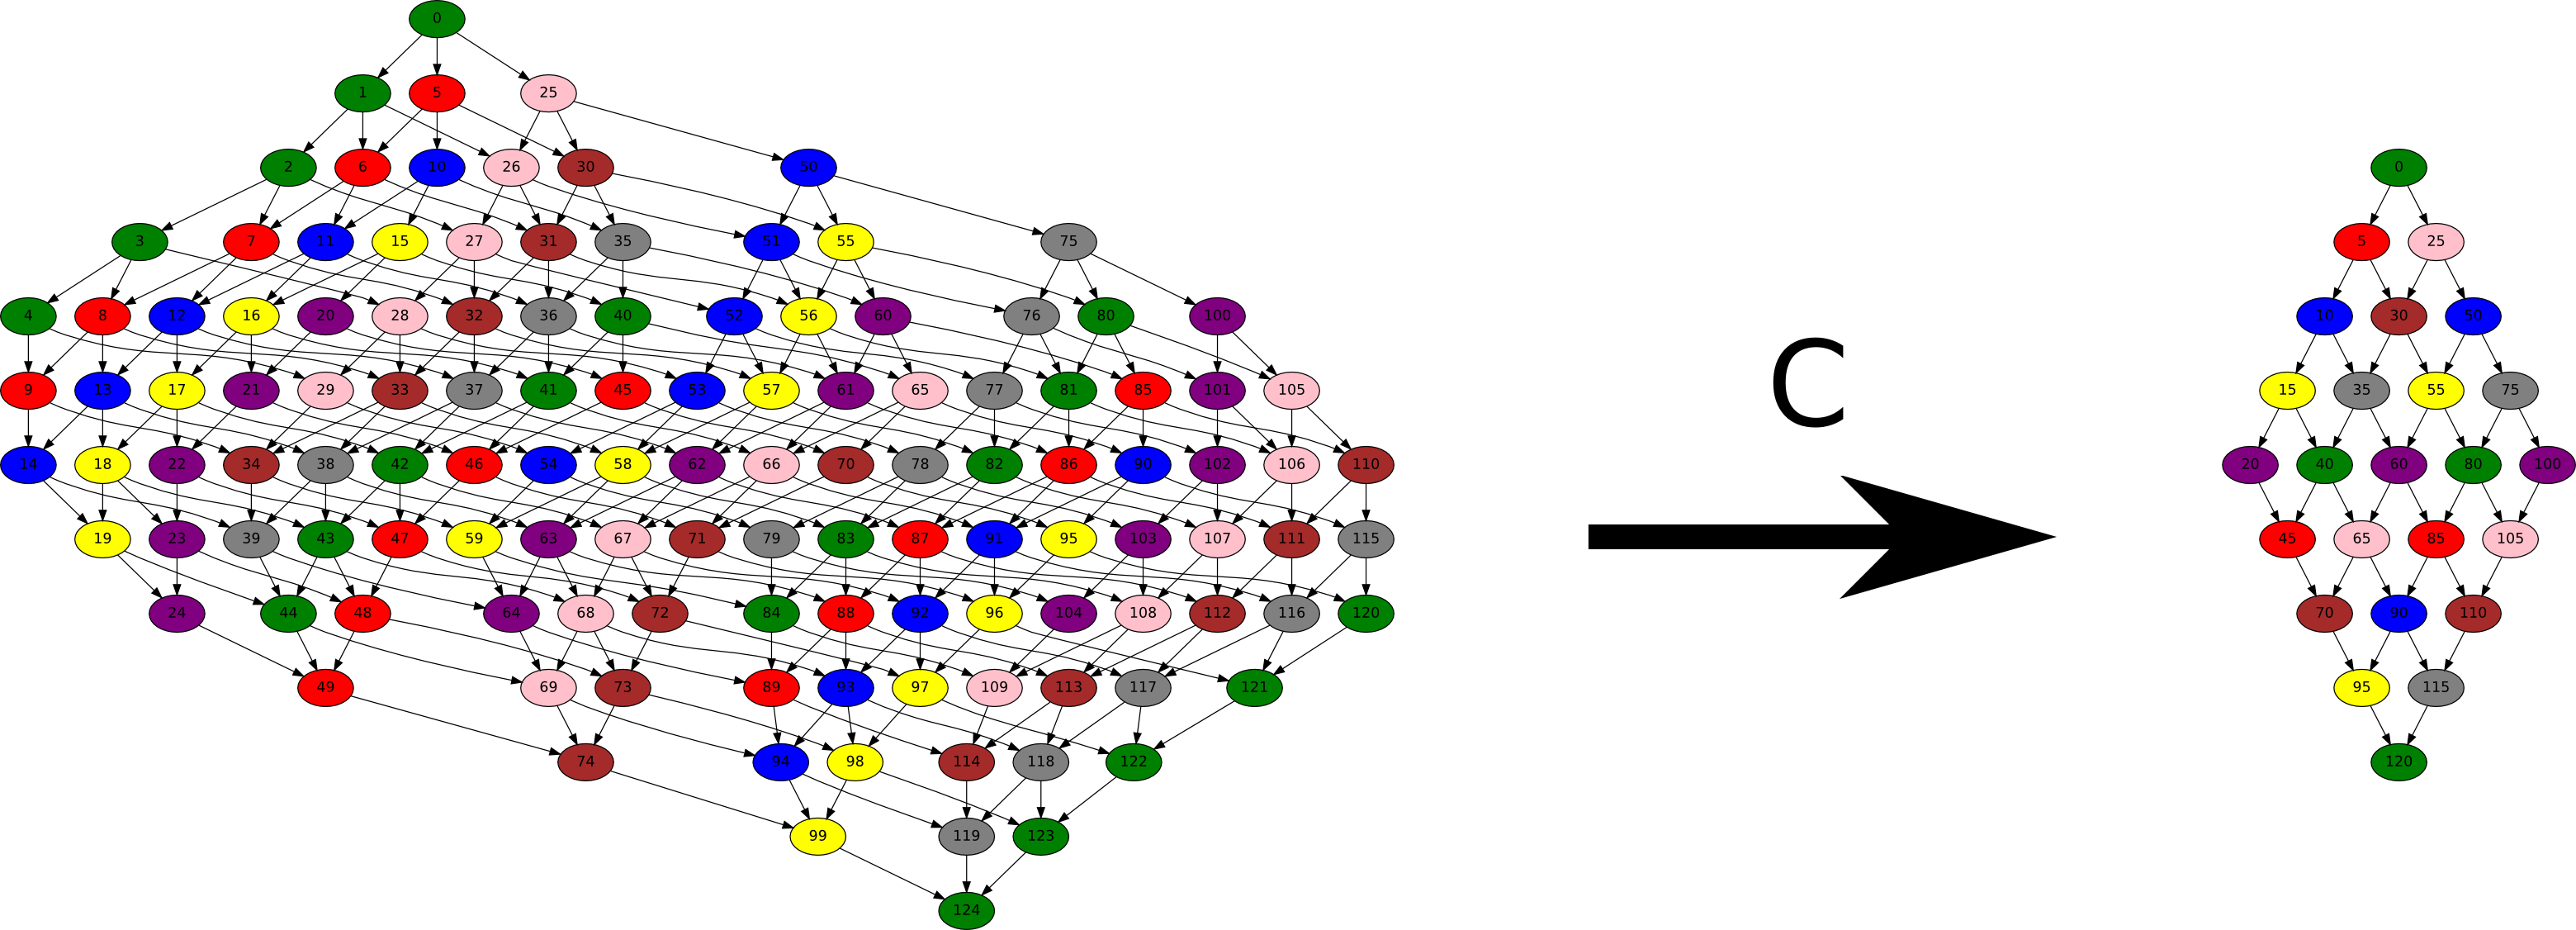
\includegraphics[width=\textwidth]{cube5_operator_c}
  \caption{Exemple d'utilisation de l'opérateur C sur un cube 5x5x5.}
  \label{fig:cube5_algo_C}
\end{figure}


%   (-_-)   %
\begin{figure}[t!]
  \centering
  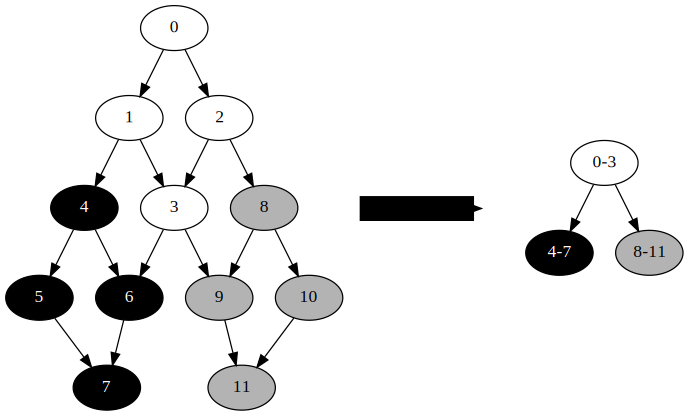
\includegraphics[width=0.8\textwidth]{algo_3}
  \caption{Exemple d'utilisation de l'opérateur C.}
  \label{fig:algo_C}
\end{figure}


Comme pour les autres opérateurs, nous devons vérifier qu'aucun cycle ne sera créé.
%
Pour fonctionner, cet opérateur a besoin que le programmeur attribue un nombre unique à chaque tâche et ainsi avoir un ordre strict sur les tâches.
%
Dans notre cas on va utiliser la numérotation naturelle des cellules.
%
Puis l'opérateur agrégera ensemble les tâches ayant des nombres qui se suivent ainsi qu'une dépendance entre les tâches.
%
Par exemple sur la figure \ref{fig:algo_C} les tâches 2 et 3 ont des nombres consécutifs mais n'ont pas de dépendance entre elles, elles ne seront donc pas agrégées ensemble.


Ajoutons un prédicat à l'algorithme : pour pouvoir utiliser cet algorithme, il faut absolument que pour chaque tâche $i$, l'indice associé à la tâche $i$ soit strictement inférieur aux indices associés aux successeurs de la tâche $i$.
%
Dans le cas d'une factorisation ILU, ce prédicat est toujours vérifié.
%
Dans le cas général, il nous permet de s'assurer qu'aucun cycle ne sera créé.
%
En effet, pour créer un cycle avec cet algorithme, il faudrait qu'il existe un chemin entre deux tâches agrégées qui passe par une autre tâche non agrégée.
%
Or, pour agréger une tâche avec une autre, il faut que la différence de leurs indices soit exactement la différence minimale possible dans le graphe.
%
Donc, en prenant en compte le prédicat, si nous agrégeons une tâche T1 avec son successeur T2, il ne peut pas exister de chemin en T1 et T2 passant par une autre tâche.


\begin{algorithm}
  \KwData{DAG}
  {\sc Pas} = Infini \\
  \For{chaque tâche {\sc T1} de DAG} {
    \For{chaque successeurs {\sc T2} de {\sc T1}} {
      \If{indice de {\sc T2} $<=$ indice de {\sc T1}} {
        \Return agrégation impossible
      }

      \If{indice de {\sc T2} - indice de {\sc T1} $<$ {\sc Pas}} {
        {\sc Pas} = indice de {\sc T2} - indice de {\sc T1}
      }
    }
  }

  \For{chaque tâche {\sc T1} de DAG} {
    \For{chaque successeurs {\sc T2} de {\sc T1}} {
      \If{indice de {\sc T2} == indice de {\sc T1} + {\sc Pas}} {
        {\sc T1} devient {\sc T1} union {\sc T2}
      }
    }
  }
  \caption{Algorithme de l'opérateur continuation.}
  \label{algo:algo_C}
\end{algorithm}

%% Dans le cas d'un graphe représentant un cube 3D, cet opérateur fonctionne très bien.
%% %
%% Par contre, dans le cas d'un graphe représentant un carré, il est nécessaire de modifier cette algorithme pour limiter la taille des agrégats tout en optimisant
